\def\colegio{Colegio Latinoamericano de Integración}
\def\titulo{Guía}
\def\subtitulo{Cuantiles y el diagrama de caja}
\def\curso{Octavo Básico}
%\def\puntaje{30}

\documentclass[sin nombre]{plantilla-evaluacion-v1}

\begin{python}
import numpy as np

def divisores(n):
    div = [i for i in range(1, int(n ** 0.5) + 1) if n % i == 0]
    div.extend([n // i for i in div if i != n // i])
    return np.array(sorted(div))

def n_barras(lista, ideal):
  if (lista is None or len(lista) == 0):
    return 0
  min = np.min(lista)
  max = np.max(lista) + 1
  rango = np.abs(max-min)
  div_rango = divisores(rango).astype(int)
  n_bars = (rango/div_rango).astype(int)
  distancia = np.abs(n_bars - ideal)
  return n_bars[distancia.argmin()]

def ticks(muestras):
  t = np.linspace(
    np.min(muestras),
    np.max(muestras)+1,
    n_barras(muestras,5)+1
  ).astype(int)
  return ",".join(t.astype(str))

def obtener_muestras(m,d,n,s=None):
  l = np.random.default_rng(seed=s).normal(m,d,size=n)
  return np.floor(l).astype(int)

muestras_h = np.array([160, 162, 160, 153, 153, 154, 157, 160, 157, 159, 155, 159, 165, 163,
  154, 165, 159, 159, 157, 156, 163, 157, 156, 155, 156, 154, 158, 159, 154, 160, 161, 153,
  158, 159, 164, 157, 155, 155, 157, 160, 154, 152, 166, 163, 158, 162, 155, 160, 157, 159],
  dtype=int)
#while (n_barras(muestras_m,5) != 5):
#  muestras_m = obtener_muestras(155,3,45)

muestras_m = np.array([153, 156, 152, 153, 152, 153, 153, 153, 153, 152, 155, 155, 152, 158,
 153, 157, 148, 153, 154, 152, 148, 158, 151, 156, 154, 150, 154, 157, 148, 155, 150, 157,
 153, 156, 154, 160, 153, 151, 154, 154, 162, 151, 157, 151, 155], dtype=int)
#while (n_barras(muestras_h,5) != 5):
#  muestras_h = obtener_muestras(158,3,50)

@np.vectorize(excluded=['lista'])
def frecuencia(x, lista):
  filtrado = np.extract(lista == x,lista)
  return len(filtrado)

@np.vectorize(excluded=['lista'])
def frecuencia_acumulada(x, lista):
  filtrado = np.extract(lista <= x, lista)
  return len(filtrado)

@np.vectorize(excluded=['lista'])
def probabilidad(x, lista):
  return frecuencia(x, lista=lista)/len(lista)

@np.vectorize(excluded=['lista'])
def probabilidad_acumulada(x, lista):
  return frecuencia_acumulada(x, lista=lista)/len(lista)

@np.vectorize(excluded=['lista'])
def cuantil(p, lista):
  unicos = np.unique_values(lista)
  dato = 0
  for i in unicos:
    p_acumulada = probabilidad_acumulada(i, lista=lista)
    if (p_acumulada >= p):
      dato = i
      break
  return dato

def pgf_coords(x,y):
  return " ".join(f"({i},{j})" for i, j in zip(x,y))

\end{python}

\begin{document}

Utilice los datos entregados para completar las tablas.

\begin{python}
#muestras1 = np.array([10,10,11,12,13],dtype=int)
muestras1 = obtener_muestras(m=10,d=4,n=5,s=4)
muestras2 = obtener_muestras(m=10,d=4,n=8,s=5)
muestras3 = obtener_muestras(m=10,d=4,n=9,s=9)
muestras4 = obtener_muestras(m=10,d=4,n=12,s=7)
muestras5 = obtener_muestras(m=10,d=4,n=15,s=8)
muestrasEjemplo = obtener_muestras(m=10,d=4,n=20,s=10)
nAmigosH = obtener_muestras(m=10,d=3,n=20,s=123)
nAmigosM = obtener_muestras(m=18,d=4,n=25,s=321)

np.savetxt("nAmigosH.csv",np.column_stack([
  x := (np.unique_values(nAmigosH)),
  frecuencia(x,lista=nAmigosH),
  frecuencia_acumulada(x,lista=nAmigosH),
  probabilidad(x,lista=nAmigosH),
  probabilidad_acumulada(x,lista=nAmigosH)
  ]),
  fmt=["%d","%d","%d","%.4f","%.4f"],
  delimiter=","
)

np.savetxt("muestrasH.csv",nAmigosH,delimiter=",")
np.savetxt("muestrasM.csv",nAmigosM,delimiter=",")

def imprimir(l):
  return ", ".join(l.astype(str))

\end{python}%
%
\newsavebox{\tabla}
\begin{lrbox}{\tabla}
  \begin{tblr}{colspec={ccccc},vlines,hlines,rowsep=6pt,colsep=10pt}
    Mínimo & 1er Cuartil ($Q_1$) & Mediana ($Q_2$) & 3er Cuartil ($Q_3$) & Máximo \\
           &                     &                 &                     &        \\
  \end{tblr}
\end{lrbox}%
%

\begin{preguntas}[after-item-skip=10pt]
  \pregunta Datos: \py{imprimir(muestras1)}.
  \begin{malla}[height=2cm]
  \end{malla}
  \begin{center}
    \usebox{\tabla}
  \end{center}

  \pregunta Datos: \py{imprimir(muestras2)}.
  \begin{malla}[height=2cm]
  \end{malla}
  \begin{center}
    \usebox{\tabla}
  \end{center}

  \pregunta Datos: \py{imprimir(muestras3)}.
  \begin{malla}[height=3cm]
  \end{malla}
  \begin{center}
    \usebox{\tabla}
  \end{center}

  \pregunta Datos: \py{imprimir(muestras4)}.
  \begin{malla}[height=3cm]
  \end{malla}
  \begin{center}
    \usebox{\tabla}
  \end{center}

  \pregunta Datos: \py{imprimir(muestras5)}.
  \begin{malla}[height=3cm]
  \end{malla}
  \begin{center}
    \usebox{\tabla}
  \end{center}

\end{preguntas}

\section*{Diagrama de caja}

Los diagramas de caja se dibujan de la siguiente manera. \par

\begin{center}
  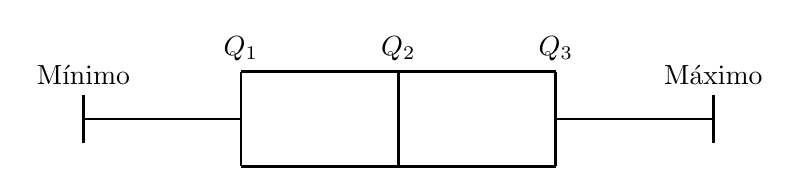
\begin{tikzpicture}[line width=1pt,x=2cm,y=0.6cm]
    \coordinate (MIN) at (0,0);
    \coordinate (Q1) at (1,0);
    \coordinate (Q2) at (2,0);
    \coordinate (Q3) at (3,0);
    \coordinate (MAX) at (4,0);

    \draw (MIN)--+(0,0.5) node [above] {Mínimo} (MIN)--+(0,-0.5);
    \draw (Q1)--+(0,1) node [above] {$Q_1$} (Q1)--+(0,-1);
    \draw (Q2)--+(0,1) node [above] {$Q_2$} (Q2)--+(0,-1);
    \draw (Q3)--+(0,1) node [above] {$Q_3$} (Q3)--+(0,-1);
    \draw (MAX)--+(0,0.5) node [above] {Máximo} (MAX)--+(0,-0.5);

    \draw (MIN)--(Q1) (Q3)--(MAX);

    \draw (Q1) +(0,1) -- (Q3 |- 1,1);
    \draw (Q1) +(0,-1) -- (Q3 |- 1,-1);
  \end{tikzpicture}
\end{center} \par

\NewDocumentCommand{\generarTabla}{m}{%
\begin{tblr}{colspec={ccccc},vlines,hlines,rowsep=6pt,colsep=10pt}
  Mínimo & 1er Cuartil ($Q_1$) & Mediana ($Q_2$) & 3er Cuartil ($Q_3$) & Máximo \\
  \py{np.min(#1)} & \py{cuantil(0.25,lista=#1)} &
  \py{cuantil(0.5,lista=#1)} & \py{cuantil(0.75,lista=#1)} &
  \py{np.max(#1)} \\
\end{tblr}}

Por ejemplo, a los datos: \py{imprimir(muestrasEjemplo)}; les corresponde la siguiente
tabla de valores. \par

\begin{center}
  \generarTabla{muestrasEjemplo}
\end{center}

Así, el diagrama de caja se ubica en un plano de la siguiente forma. \par
\begin{python}
coordenadasEjemplo = [f"(0,{x})" for x in muestrasEjemplo]
\end{python}

\begin{center}
  \begin{tikzpicture}
    \begin{axis}[width=0.7\linewidth,height=4cm,boxplot/box extend = 0.4,ymin=0.6,ymax=1.4,
      hide y axis,axis x line=bottom,enlarge x limits,xlabel={Datos}]
      \addplot+ [boxplot] coordinates {\py{" ".join(coordenadasEjemplo)}};
    \end{axis}
  \end{tikzpicture}
\end{center}

\section*{Comparando el número de amistades por género}

A continuación, se encuentran los resultados de encuestar a un grupo de estudiantes y
preguntarles a cada uno: \textbf{¿Cuántos amigos tienes?}. \par

Los resultados se encuentran separados por género. Para las niñas, los datos se encuentran
en una tabla de frecuencias; y para los niños, los datos se encuentran en un gráfico de barras.
Utilice estos valores para completar la tabla de valores de cada género, y así finalmente
dibujar dos diagramas de caja comparando el número de amistades por género.

\NewDocumentCommand{\formatear}{m}{\pgfmathprintnumber[fixed,fixed zerofill,precision=3,verbatim,use comma]{#1}}
\csvreader[no head,
%before reading=\pgfkeys{/pgf/number format/.cd,fixed,fixed zerofill,precision=3,verbatim,use comma},
centered tabularray={
cells={valign=m},
colspec={X[1,c]X[2,c]X[2,c]X[2,c]X[2,c]},
width=0.7\linewidth,
hlines,
vlines,
hline{1,2,3,Z}={black,1pt},
rows={rowsep+=2pt},
cell{1}{1}={r=1,c=5}{c}
},
table head={Número de amig@s (Niños) & F & FA & P & PA \\ Datos & Frecuencia &
  {Frecuencia\\Acumulada} & Probabilidad & {Probabilidad\\Acumulada} \\}
]{nAmigosH.csv}{1=\a, 2=\b, 3=\c, 4=\d, 5=\e}%
{\a & \b & \c & \formatear{\d} & \formatear{\e} }

\begin{preguntas}(1)
  \pregunta Complete la tabla de valores usando las respuestas de los niños. \\[5pt]
  \usebox{\tabla}
\end{preguntas}%
%
\begin{python}
x_m = np.unique_values(nAmigosM)
y_m = frecuencia(x_m,lista=nAmigosM)
\end{python}%
%
\begin{center}
  \vspace*{1cm}
  \begin{tikzpicture}[baseline=(current axis.north)]
    \begin{axis}[
        ybar,
        title={Número de amig@s (Niñas)},
        ylabel={Frecuencia},
        xlabel={Número de amig@s},
        xtick distance=3,
        ymin=0,
        %xtick=data,
        %nodes~near~coords,
        %nodes~near~coords~align={vertical},
        ]
        \addplot [ybar,bar width=1,pattern={Lines[angle=-45,distance=5pt]}]
         coordinates {\py{pgf_coords(x_m,y_m)}};
    \end{axis}
  \end{tikzpicture}
\end{center}

\begin{preguntas}[after-item-skip=20pt](1)
  \pregunta Complete la tabla de valores usando las respuestas de las niñas.\\[5pt]
  \begin{malla}[height=3cm]
  \end{malla}
  \usebox{\tabla}
  \pregunta Usa los datos de ambos grupos para dibujar los diagramas en el espacio
  señalizado. \\[5pt]
  \begin{center}
    \begin{tikzpicture}[baseline=(current axis.north)]
      \begin{axis}[
        title={Número de amig@s por grupo},
        xlabel={Número de amig@s},
        ytick={1,2},
        yticklabels={Niñas,Niños},
        width=0.85\linewidth,
        height=5cm,
      ]
        \addplot+ [boxplot={
          draw position=1,
          whisker range=10,
        },draw=white] table[y index=0] {muestrasM.csv};
        \addplot+ [boxplot={
          draw position=2,
          whisker range=10,
        },draw=white] table[y index=0] {muestrasH.csv};
      \end{axis}
    \end{tikzpicture}
  \end{center}
  \pregunta Según los datos, ¿Qué grupo tiene más amig@s? Justifique
  su respuesta usando los diagramas de caja de cada grupo.
  \begin{respuesta}[height=4cm]
  \end{respuesta}
\end{preguntas}



\newpage
\begin{minipage}[c][\lineskip+20pt][c]{\linewidth}
  \centering
  \sffamily\Large {\scshape\bfseries Respuestas} - \subtitulo
\end{minipage}

\begin{preguntas}[resume=false,after-item-skip=10pt]
  \pregunta \generarTabla{muestras1}
  \pregunta \generarTabla{muestras2}
  \pregunta \generarTabla{muestras3}
  \pregunta \generarTabla{muestras4}
  \pregunta \generarTabla{muestras5}
  \pregunta \generarTabla{nAmigosH}
  \pregunta \generarTabla{nAmigosM}
  \pregunta
  \begin{center}
    \begin{tikzpicture}[baseline=(current axis.north)]
      \begin{axis}[
        title={Número de amig@s por grupo},
        xlabel={Número de amig@s},
        ytick={1,2},
        yticklabels={Niñas,Niños},
        width=0.8\linewidth,
        height=5cm,
      ]
        \addplot+ [boxplot={
          draw position=1,
          whisker range=10,
        }] table[y index=0] {muestrasM.csv};
        \addplot+ [boxplot={
          draw position=2,
          whisker range=10,
        },solid] table[y index=0] {muestrasH.csv};
      \end{axis}
    \end{tikzpicture}
  \end{center}
\end{preguntas}



\end{document}